% MultiCogTrust model architecture: audio-text cross-modal fusion (model B) with late face fusion.
% Build: latexmk -pdf architecture.tex   (standalone; \includegraphics the PDF in a paper)
\documentclass[tikz,border=4pt]{standalone}
\usepackage[T1]{fontenc}
\usepackage{lmodern}
\usepackage{amsmath}
\usetikzlibrary{arrows.meta,positioning,fit,calc,backgrounds}

% "text" is a TikZ key, so the stream colours carry a suffix.
\definecolor{audiocol}{HTML}{1A7F63}
\definecolor{textcol}{HTML}{2A62C4}
\definecolor{facecol}{HTML}{B4621A}

\tikzset{
  block/.style={draw, rounded corners=2pt, align=center, font=\small, fill=white,
                minimum height=10mm, inner xsep=5pt, inner ysep=3pt},
  frozen/.style={block, fill=gray!12},
  feat/.style={font=\small, inner sep=2pt, align=center},
  flow/.style={-{Stealth[length=2.2mm]}, line width=0.7pt},
  note/.style={font=\scriptsize\itshape, text=black!60},
  group/.style={draw=black!45, dashed, rounded corners=4pt, inner sep=7pt},
}

\begin{document}
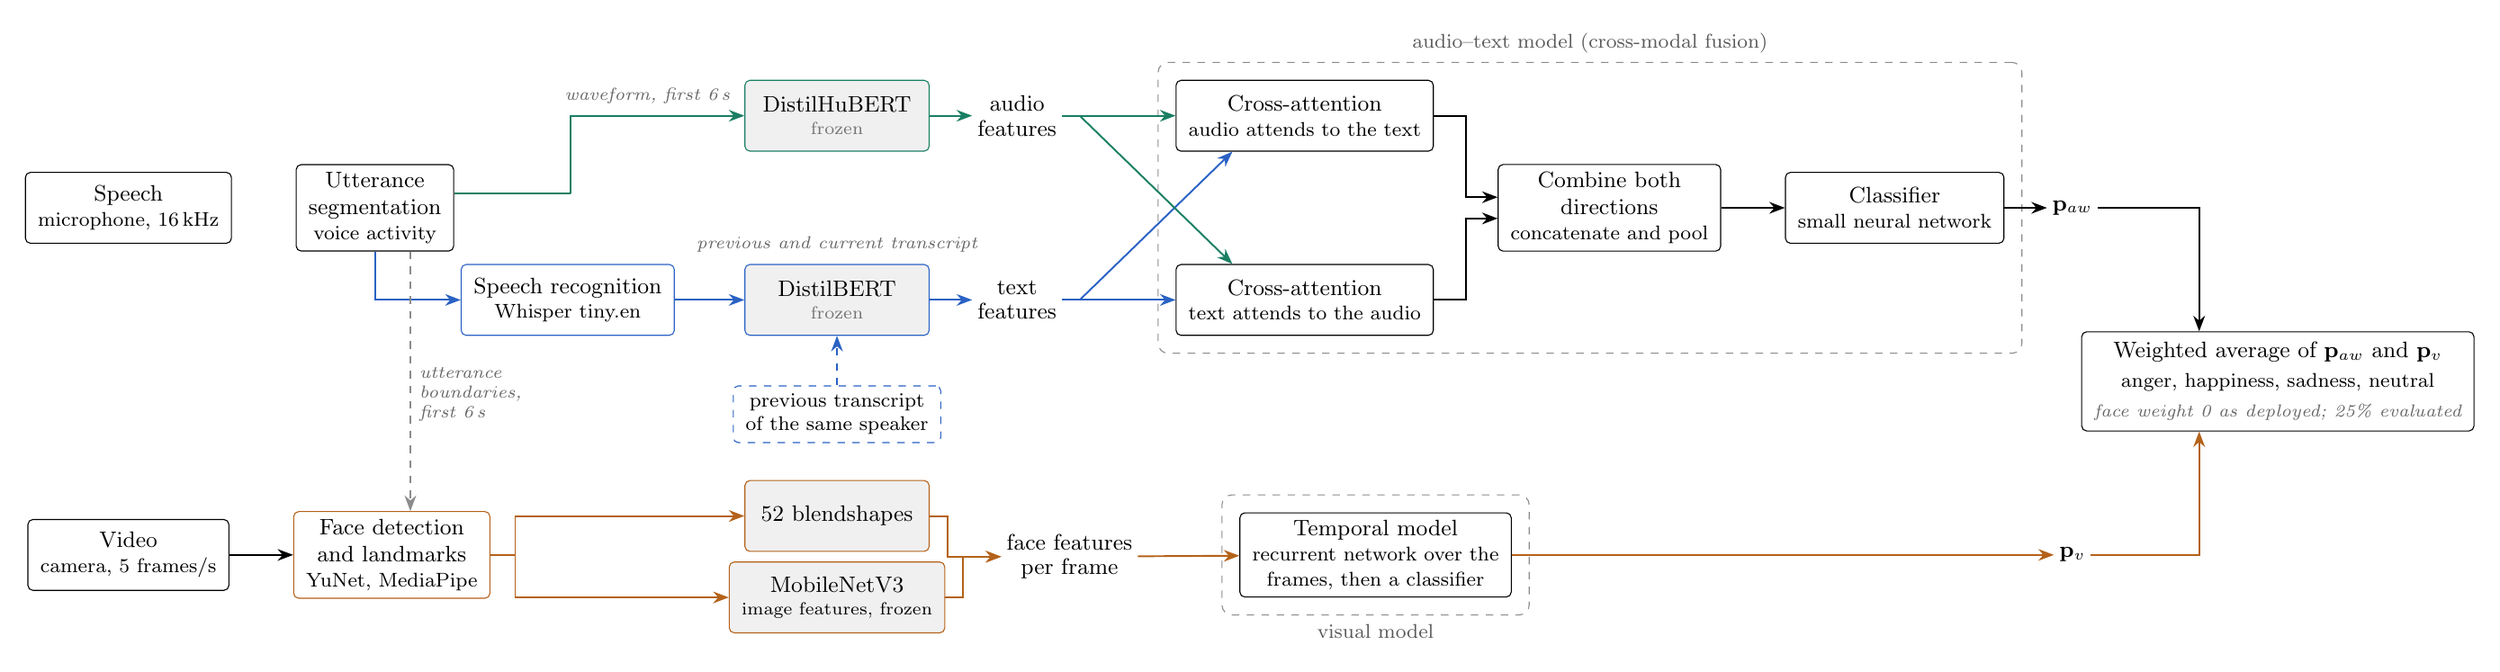
\begin{tikzpicture}[node distance=6mm and 9mm]

  % ---- Speech, segmented into utterances ---------------------------------------------------
  \node[block] (speech) at (0, 1.3) {Speech\\[-1pt]{\footnotesize microphone, 16\,kHz}};
  \node[block, right=of speech] (vad) {Utterance\\segmentation\\[-1pt]{\footnotesize voice activity}};

  % audio row
  \node[frozen, draw=audiocol, minimum width=26mm] (hubert) at (10.0, 2.6) {DistilHuBERT\\[-2pt]\textcolor{black!55}{\scriptsize frozen}};
  \node[feat, right=6mm of hubert] (Ha) {audio\\[-1pt]features};
  \draw[flow, audiocol] ($(vad.east)+(0,0.2)$) -| ($(vad.east)!0.4!(hubert.west |- vad.east)+(0,0.2)$) |- (hubert.west);
  \node[note, anchor=south east] at ($(hubert.west)+(-0.08,0.04)$) {waveform, first 6\,s};

  % text row: the current transcript, preceded by the speaker's previous one
  \node[block, draw=textcol] (asr) at (6.2, 0.0) {Speech recognition\\[-1pt]{\footnotesize Whisper tiny.en}};
  \node[frozen, draw=textcol, minimum width=26mm] (bert) at (10.0, 0.0) {DistilBERT\\[-2pt]\textcolor{black!55}{\scriptsize frozen}};
  \node[feat, right=6mm of bert] (Hw) {text\\[-1pt]features};
  \draw[flow, textcol] (vad.south) |- (asr.west);
  \draw[flow, textcol] (asr) -- (bert);
  \node[block, dashed, draw=textcol, font=\footnotesize, minimum height=8mm, below=7mm of bert] (ctx)
       {previous transcript\\of the same speaker};
  \draw[flow, textcol, dashed] (ctx) -- (bert);
  \node[note, anchor=south] at ($(bert.north)+(0,0.04)$) {previous and current transcript};

  \draw[flow, audiocol] (hubert) -- (Ha);
  \draw[flow, textcol] (bert) -- (Hw);

  % ---- Cross-modal fusion -----------------------------------------------------------------
  \node[block, minimum width=34mm] (ca1) at (16.6, 2.6) {Cross-attention\\[-1pt]{\footnotesize audio attends to the text}};
  \node[block, minimum width=34mm] (ca2) at (16.6, 0.0) {Cross-attention\\[-1pt]{\footnotesize text attends to the audio}};
  \draw[flow, audiocol] (Ha.east) -- (ca1.west |- Ha.east);
  \draw[flow, textcol]  (Hw.east) -- (ca2.west |- Hw.east);
  \draw[flow, textcol]  ($(Hw.east)+(0.25,0)$) -- ($(ca1.south west)!0.22!(ca1.south east)$);
  \draw[flow, audiocol] ($(Ha.east)+(0.25,0)$) -- ($(ca2.north west)!0.22!(ca2.north east)$);

  \node[block] (pool) at (20.9, 1.3) {Combine both\\directions\\[-1pt]{\footnotesize concatenate and pool}};
  \node[block, right=of pool] (mlp) {Classifier\\[-1pt]{\footnotesize small neural network}};
  \node[feat, right=6mm of mlp] (paw) {$\mathbf{p}_{aw}$};
  \draw[flow] (ca1.east) -| ($(ca1.east)!0.5!(pool.west |- ca1.east)$) |- ($(pool.west)+(0,0.15)$);
  \draw[flow] (ca2.east) -| ($(ca2.east)!0.5!(pool.west |- ca2.east)$) |- ($(pool.west)-(0,0.15)$);
  \draw[flow] (pool) -- (mlp);
  \draw[flow] (mlp) -- (paw);

  % ---- Face -------------------------------------------------------------------------------
  \node[block] (video) at (0, -3.6) {Video\\[-1pt]{\footnotesize camera, 5 frames/s}};
  \node[block, right=of video, draw=facecol] (facedet) {Face detection\\and landmarks\\[-1pt]{\footnotesize YuNet, MediaPipe}};
  \node[frozen, draw=facecol, minimum width=26mm] (blend) at (10.0, -3.05) {52 blendshapes};
  \node[frozen, draw=facecol, minimum width=26mm] (mobile) at (10.0, -4.2) {MobileNetV3\\[-2pt]{\scriptsize image features, frozen}};
  \node[feat, right=9mm of $(blend.east)!0.5!(mobile.east)$] (f) {face features\\[-1pt]per frame};
  \node[block, minimum width=34mm] (gru) at (17.6, -3.6) {Temporal model\\[-1pt]{\footnotesize recurrent network over the}\\[-1pt]{\footnotesize frames, then a classifier}};
  \node[feat] (pv) at (paw |- gru) {$\mathbf{p}_{v}$};
  \draw[flow] (video) -- (facedet);
  \draw[flow, facecol] (facedet.east) -- ++(0.35,0) |- (blend.west);
  \draw[flow, facecol] ($(facedet.east)+(0.35,0)$) |- (mobile.west);
  \draw[flow, facecol] (blend.east) -- ++(0.25,0) |- (f.west);
  \draw[flow, facecol] (mobile.east) -- ++(0.25,0) |- (f.west);
  \draw[flow, facecol] (f) -- (gru);
  \draw[flow, facecol] (gru) -- (pv);
  % frames are taken within the utterance found on the speech side
  \draw[flow, black!45, dashed] ($(vad.south)+(0.5,0)$) -- ($(vad.south |- facedet.north)+(0.5,0)$)
       node[pos=0.55, right, note, align=left] {utterance\\boundaries,\\first 6\,s};

  % ---- Late fusion ------------------------------------------------------------------------
  \node[block, minimum height=14mm] (late) at ($(paw)!0.5!(pv) + (2.9,0)$)
       {Weighted average of $\mathbf{p}_{aw}$ and $\mathbf{p}_{v}$\\[1pt]{\footnotesize anger, happiness, sadness, neutral}\\[1pt]
        {\scriptsize\itshape\color{black!60} face weight 0 as deployed; 25\% evaluated}};
  \draw[flow] (paw.east) -| ($(late.north west)!0.3!(late.north east)$);
  \draw[flow, facecol] (pv.east) -| ($(late.south west)!0.3!(late.south east)$);

  % ---- Groups -----------------------------------------------------------------------------
  \begin{scope}[on background layer]
    \node[group, fit=(ca1)(ca2)(pool)(mlp), label={[font=\footnotesize, text=black!65]above:audio--text model (cross-modal fusion)}] {};
    \node[group, fit=(gru), label={[font=\footnotesize, text=black!65]below:visual model}] {};
  \end{scope}
\end{tikzpicture}
\end{document}
